
The general constraint we can impose on an interface is that the momentum flow (or current flow if exists) should be continuous. An equivalent way of viewing it (and will be used later) is to fold one of the theories on top of the other. The interface now located on the boundary of the tensor theory becomes impenetrable, and momentum flow ends there. This folding picture leads to the concept of boundary states in the framework of boundary CFT\cite{cardy_boundary_2004,cardy_conformal_1984}. In the Boson theory we are interested in, the tensor theory has $c = 2$ and the general classification the boundary state is still an open questions\cite{affleck_quantum_2001}. 

There are however many successful attempts to construct a subset of those bosonic boundary states. One way is to impose current operator rather than Virasoro generator constraints, which dates back to the idea of the Ishibashi state\cite{ishibashi_boundary_1989} and can be applied to the multi-component boson with a general compactification lattice\cite{affleck_quantum_2001,oshikawa_boundary_2010,quella_reflection_2007}. Other examples utilize the fusion algebra to generate new boundary states from the known ones\cite{affleck_quantum_2001,bachas_fusion_2008}. 

We here follow the presentation in Ref.~\onlinecite{bachas_permeable_2002} that begins with a classical boundary condition and then quantizes it to give the boundary state. The interface obtained is actually the same as using the current algebra constraints\cite{affleck_quantum_2001,oshikawa_boundary_2010,quella_reflection_2007}, but we feel that scattering process derived here and its relation to the discrete lattice model in Sec.~\ref{sec_sub:free_boson_lattice} are more intuitive. 

Assume two free Bosons fields $\phi^1$ and $\phi^2$ live on the left and right half planes respectively. Their interface located at $x = 0$ are characterized by the ``gluing condition"
\begin{equation}\begin{aligned}
\label{eq:def_M}
\begin{pmatrix}
\partial_t\phi^1\\
\partial_x\phi^1
\end{pmatrix}
=M\begin{pmatrix}
\partial_t\phi^2\\
\partial_x\phi^2
\end{pmatrix}
\end{aligned}\end{equation}
where derivative should be understood in the appropriate left and right limits, for example $\partial_x \phi^1$ is evaluated at $ x = 0^-$. As argued, the momentum component of stress tensor is continuous across the interface. As a consequence $M$ is an element of the Lorentz group $O(1,1)$ and can be parameterized as
\begin{equation}\begin{aligned}
\label{eq:M1M2}
M_1(\theta)=\pm
\begin{bmatrix}
\lambda^{-1} & 0 \\
0 & \lambda
\end{bmatrix}\quad
M_2(\theta)=\pm
\begin{bmatrix}
0 & \lambda  \\
\lambda^{-1} & 0 
\end{bmatrix}
\end{aligned}\end{equation}
where $\lambda=\tan\theta$ for $\theta\in\left[-\frac{\pi}{2},\frac{\pi}{2}\right]$. 

Several special choices of $\theta$ need to be noted. 
\begin{enumerate}
\item $\theta=0,\pm \frac{\pi}{2}$. In this case, $\lambda$ (or $\lambda^{-1}$) appears to be singular and the field on either side of the interface cannot transmit to the other. The interface reduces to individual boundary conditions for the boson on the left and right half planes: they are combination of Dirichlet and Neumann boundary conditions. For example, $\lambda = 0$ for $M_1$ implies $\partial_x\phi^1 = \partial_t\phi^2 =0$, which means that Dirichlet boundary condition is imposed on the right and Neumann boundary condition on the left. Hereafter we shall denote this combination as `DN'. Similarly $M_1(\pm\frac{\pi}{2}),M_2(0),M_2(\pm \frac{\pi}{2})$ correspond to `ND', `DD', `NN' respectively. 
\item $\theta = \pm \frac{\pi}{4}$. In this case, $M_1(\theta)$ characterizes a perfectly transmitting interface. For example, there is effectively no interface in the case $M_1( \frac{\pi}{4})$ which is the traditional periodic boundary condition and we will denote it as P. For the other three cases, despite picking up a phase, the two counter propagating modes are still fully transmitted cross the interface. 
\end{enumerate}

The physical significance of $\theta$ will be manifest in the scattering process described below. We rewrite the Eq.~\eqref{eq:def_M} in the coordinates $t\pm x$ and use $\partial_{\pm} = \partial_{t} \pm \partial_x $ to extract the left and right going modes. For example, $\partial_{-} \phi^2$ will be a function $t - x$ and hence represents a right going mode on the right half plane. It is then one of the scattering products that leaves the interface. On the other hand $\partial_{-} \phi^1$ and $\partial_{+} \phi^2$ are modes that approaching the interface from their respective domain. We therefore establish the scattering relation 
\begin{equation}\begin{aligned}
\label{eq:def_S}
\begin{pmatrix}
\partial_+\phi^1\\
\partial_-\phi^2
\end{pmatrix}
=S
\begin{pmatrix}
\partial_-\phi^1\\
\partial_+\phi^2
\end{pmatrix}
\end{aligned}\end{equation}
and solve the $S$ matrix for the two cases of $M_1$ and $M_2$
\begin{equation}\begin{aligned}
\label{eq:S1_S2}
S_1(\theta)=\begin{bmatrix}
\cos 2\theta & \sin 2\theta \\
\sin 2\theta & -\cos 2\theta
\end{bmatrix}\quad
S_2(\theta)=\begin{bmatrix}
-\cos 2\theta & \sin 2\theta \\
-\sin 2\theta & -\cos 2\theta
\end{bmatrix}
\end{aligned}\end{equation}
For generic values of $\theta$, the interface is partially-transmitting, whose transmission and reflection coefficients can be read off from the scattering matrices. The fact of their wavelength independence is an indication of scale invariance of the interface.

\begin{figure}[h]
\centering
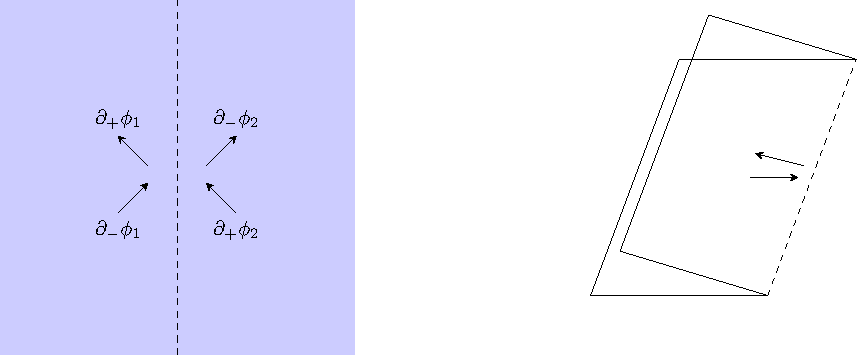
\includegraphics[width=0.5\textwidth]{fig_folding_pic.pdf}
\caption{Folding picture for penetrable interface. Left panel: World line of the penetrable interface. $\partial_\pm\phi^{1,2}$ denote the left and right going modes in their respective domain. Right panel: Folding operation that sends $\phi^2(x)$ to $\phi^2(-x)$. The dashline represents the \emph{im}penetrable boundary for the resulting tensor theory.}
\label{fig:folding_pic}
\end{figure}

We now work in the folding picture as shown in Fig.~\ref{fig:folding_pic}. The boundary at $x=0$ becomes impenetrable for the folded system, and the resulting tensor theory admits a conformal boundary state. The folding sends $\phi^2(x)$ to $\phi^2(-x)$ and hence the gluing condition becomes
\begin{equation}
\begin{aligned}
\partial_t(\sin\theta\phi^1-\cos\theta\phi^2)=0 \quad
\partial_x(\cos\theta\phi^1+\sin\theta\phi^2)=0 
\end{aligned}
\end{equation}
for the case $M = M_1(\theta)$. 

If we quantize the Boson theory on the interface line $x = 0$, these gluing conditions become an operator identity for the boson creation and annihilation of the modes. We shall interpret these identities to be valid only when acting on the boundary states. The mode expansion of free boson on $x = 0$\cite{di_francesco_conformal_1997} is
\begin{equation}
\phi(z, \bar{z} ) = \phi_0 - \frac{i}{4\pi g } \pi_0 \ln z \bar{z}  + \frac{i}{\sqrt{4\pi g} } \sum_{n \ne 0 } \frac{1}{n} \left(a_n z^{-n} + \bar{a}_{n} \bar{z}^{-n}   \right)
\end{equation}
where we take $T$ to be time period and the following choice of the holomorphic and anti-holomorphic coordinates
\begin{equation}
z= e^{ \frac{2\pi i(x - t)}{T} } \quad \bar{z} = e^{ \frac{2\pi i( x + t  )}{T} }
\end{equation}
We end up with a set of operator identities for each mode
\begin{equation}
\begin{aligned}
\label{eq:rotation_a_basis}
\sin  \theta a^1_n - \cos \theta a^2_n  &= + \left( \sin  \theta \bar{a}^1_{-n} - \cos \theta \bar{a}^2_{-n} \right)\\
\cos  \theta a^1_n + \sin \theta a^2_n  &= - \left( \cos  \theta \bar{a}^1_{-n} + \sin \theta \bar{a}^2_{-n} \right) 
\end{aligned}
\end{equation}
which is valid on the following boundary state
\begin{equation}
\label{eq:bd_state}
\begin{aligned}
| B \rangle 
& =  \exp\Big\{ -\sum_{n > 0 } \frac{1}{n}
\begin{pmatrix}
a_{-n}^1\\
a_{-n}^2\\                              
\end{pmatrix}
S_1( \theta )
\begin{pmatrix}
\bar{a}_{-n}^1  \bar{a}_{-n}^2
\end{pmatrix} \Big\} |0\rangle
\end{aligned}
\end{equation}
where $S_1(\theta) $ is precisely the scattering matrix in Eq.~\eqref{eq:def_S}. The calculation for the case $M=M_2(\theta)$ is completely analogous. 

The boundary state expression in Eq.~\eqref{eq:bd_state} will be used extensively in fidelity and Loschmidt echo calculation in Sec.~\ref{sec:analytic_numerics}. 

%%% Local Variables:
%%% TeX-master: "bCFT_paper"
%%% TeX-PDF-mode: t
%%% End:
